%\newpage

\section{Examples of scale approximations for \CL models \la{ex:1}}

In this section, examples along with numerical simulations will be presented. We plot the graphs \re{of $W_q$, and also of $W'_q$, $W''_q$, when they exhibit oscillations}, and determine the "winning approximation" \wrt the exact solution. We consider the \CL\ model with exponential mixtures of jumps (in this case, the computation of $W_q,Z_q$ is fast and error-less with symbolic algebra systems, since it belongs to the realm of rational computations).

\re{\Ito the \deV\  of $\Fq$ is always the best, but Renyi may also win  occasionally when approximating $b_{DeF}$ -- see  ...}


\subsection{A Cram\'{e}r-Lundberg process with hyperexponential claims of order 3} \label{e:MixExp83}
Consider a Cram\'{e}r-Lundberg process with density function
$f(x)=\frac{12}{83 }e^{-x}+\frac{42}{83} e^{-2 x}+\frac{150}{83}e^{-3x}$, and $c=1$,  $\l=\frac{83}{48}$, $\th=\fr{263}{235}$, $p= \fr{263}{498}$, $q=\fr{5}{48}$.

\iffalse
In  figure \ref{f:MEp1}, we draw the exact \rp, together with the \deV\ and
Renyi  and the $\s >0$  approximation from section \ref{s:sp}, where the values of $\mu,\l,c,\s$ are obtained by four moments fitting, as  in \eqr{ap3}.

\figu{MEp1}{The  approximations are practically indistinguishable for large $x$ of the exact formula  for $f(x)=\frac{12}{83 }e^{-x}+\frac{42}{83} e^{-2 x}+\frac{150}{83}e^{-3x}$. They make total integrated errors of $0.0117649, 0.00939695, 0.0138467$, with \deV\ winning.}{}

At a heuristic level,  the explanation lies in the fact that the exact \rp\ is  less oscillating than the initial density (the exact \rp\ is a smoother!), in the sense that the contribution of the non-dominant exponentials is decreased,
and  even the simplest
 approximations by one  exponential work very well.

\fn[4]{This was produced by taking
$\Fq=\frac{1}{3}, c=1$ and
a negative Wiener-Hopf factor
$$\f_-(s)=\frac{\left(\frac{s}{3}+1\right) \left(\frac{s}{2}+1\right) (s+1)}{\left(\frac{2 s}{5}+1\right) \left(\frac{2 s}{3}+1\right) (2
   s+1)}$$
   with poles $-\fr 1 2, -\fr 3 2, -\fr 5 2$.}

\fi

The Laplace exponent of this process is
$\kappa(s) = s - \frac{12 s}{83 (s+1)}-\frac{21 s}{83 (s+2)}-\frac{50 s}{83 (s+3)}$ and from this one can invert $\frac{1}{\kappa(s) - q} =  \H{W}_q(s)$ to obtain the scale function \footnote{Laplace inversion done via Mathematica; coefficients and exponents are decimal approximations of the real values.}
\bea
W_q(x)  &= -0.0813294 e^{(-2.60997 x)} - 0.179472 e^{(-1.68854 x)} - 0.373887 e^{(-0.779311 x)}  + 1.63469 e^{(0.18198 x)}.
\eea

From this, we see that the dominant exponent is $\Phi_q = 0.18198$. The unique minimum of $W_q'$ is at $b_{DeF}=1.89732$, and we conclude that this is the optimal barrier that  maximizes dividends.

Figure \ref{fig:MixExp83} shows the plots of $W_q$ as well as its first two derivatives. The plots of the exact $W_q$ and its derivatives are labelled Wxexact, and coloured as the darkest. The plot of $W_q'$ an exhibits the noticeable minimum around \red{$x=1.9$}.%, and is supported by the fact that $W_q''$ has a zero at around the same point.

\begin{figure}[!h]
    \centering
    \begin{subfigure}[b]{0.8\textwidth}
        \includegraphics[width=\textwidth]{MixExp83W.eps}
        \caption{$W_q(x)$  (in black)}
        \label{fig:MixExp83W}
    \end{subfigure}
    ~
    \\
    \begin{subfigure}[b]{0.8\textwidth}
        \includegraphics[width=\textwidth]{MixExp83W1}
        \caption{$W'_q(x)$}
        \label{fig:MixExp83W1}
    \end{subfigure}
    ~
    \\
    \begin{subfigure}[b]{0.8\textwidth}
        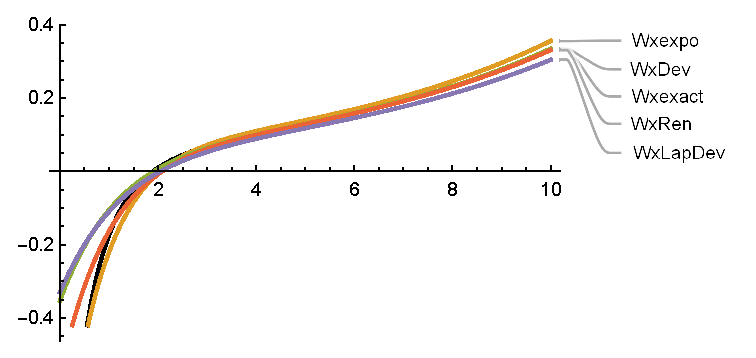
\includegraphics[width=\textwidth]{MixExp83W2}
        \caption{$W''_q(x)$}
        \label{fig:MixExp83W2}
    \end{subfigure}
    \caption{Plots of $W_q(x)$, $W'_q(x)$, and $W''_q(x)$ of the exact solution and the approximations for $f(x)=\frac{12}{83 }e^{-x}+\frac{42}{83} e^{-2 x}+\frac{150}{83}e^{-3x}$, $c=1$, $q=\fr{5}{48}$.}\label{fig:MixExp83}
\end{figure}

Continuing, from the parameters of the process, one can obtain the approximations to the scale function $W_q$ as described in the earlier section. Table \ref{table:MixExp83} gives a summary of the values of $\Phi_q$ and $b_{DeF}$ obtained from these approximations, as well as the relative errors %each one's percent deviation 
from the exact value. \footnote{Percent relative error is computed as the absolute value of the difference between the approximation and the exact, divided by the exact value, times 100. Differences in values when computed from the table and the displayed value may be explained by rounding off errors.}
We can observe a relative error  of less than $2\%$ for each of the approximations' $\Phi_q$ value, with the DeVylder approximation's $\Phi_q$ beating the others. %Considering the optimal barrier $b_{DeF}$ obtained from each, we observe only the DeVylder approximation's $b_{DeF}$ to have a relative error  of less than $7 \%$.

We also tried varying the safety loading factor $\theta$, keeping the density $f$ and the discount rate $q$ to be the same. Over certain values of $\theta \in [0, 263/235]$ we observe the trend of the DeVylder approximation exhibiting the least relative error  in approximating $\Phi_q$. Though the DeVylder approximations displayed increasing errors for decreasing values of $\theta$, the errors never went above $2\%$. A table summarizing the results can be found at table \ref{table:MixExp83Phiq}. Unlike this observation for $\Phi_q$, we are unable to conclude anything when looking at the approximate values for $b_{DeF}$. For $\theta=43/235, 23/235, 3/235$, all of the approximations yielded $b_{DeF}=0$ as the optimal barrier. This turned out to be true for $\theta=3/235$.
\beR {Note (see \fe \cite[Sec. 3]{AGV}) that the necessary, and in our case sufficient condition for the nonnegativity of the optimal dividends barrier is $W_{\q}'' (0_+) <0 \Eq (\frac {\lambda+ \q }  c )^2 < \frac {\lambda}  c f(0)$. Here, this condition is \satd\ for   the exact when $\th \geq ...$. For the approximations, it is \satd\ at ...  }
\eeR

\begin{table}[!h]
\begin{tabular}{|l|l|l|l|l|}
\hline
       & \begin{tabular}[c]{@{}l@{}}Dominant   exponent \\ $\Phi_q$\end{tabular} & \begin{tabular}[c]{@{}l@{}}Percent   relative error\\ ($\Phi_q$)\end{tabular} & \begin{tabular}[c]{@{}l@{}}Optimal barrier\\ $b_{DeF}$\end{tabular} & \begin{tabular}[c]{@{}l@{}}Percent   relative error\\ ($b_{DeF}$)\end{tabular} \\ \hline
Exact  & 0.18198                                                               & 0                                                                           & 1.89732                                                      & 0                                                                       \\ \hline
Expo   & 0.184095                                                              & 1.162215628                                                                 & 2.04608                                                      & 7.840532962                                                             \\ \hline
Dev    & 0.182011                                                              & 0.017034839                                                                 & 1.91233                                                      & 0.79111589                                                              \\ \hline
Renyi  & 0.181708                                                              & 0.149466974                                                                 & 2.08136                                                      & 9.699997892                                                             \\ \hline
LapDev & 0.178939                                                              & 1.671062754                                                                 & 2.04661                                                      & 7.868467101                                                             \\ \hline
\end{tabular}
\caption{Exact and approximate values of $\Phi_q$ and $b_{DeF}$ for $f(x)=\frac{12}{83 }e^{-x}+\frac{42}{83} e^{-2 x}+\frac{150}{83}e^{-3x}$, $c=1$, $q=\fr{5}{48}$. The DeVylder approximation displayed the least relative error  among the four approximations considered.}
\label{table:MixExp83}
\end{table}

\begin{table}[!h]
\begin{tabular}{|l|l|l|l|l|}
\hline
$\theta$ & Closest approximation & $\Phi_q$   exact & $\Phi_q$ approximation & \% error   $\Phi_q$ \\ \hline
263/235    & Dev                   & 0.18198        & 0.182011      & 0.0168217         \\ \hline
243/235    & Dev                   & 0.194712       & 0.194754      & 0.0213671         \\ \hline
223/235    & Dev                   & 0.209221       & 0.209279      & 0.0274827         \\ \hline
203/235    & Dev                   & 0.225876       & 0.225957      & 0.0358309         \\ \hline
183/235    & Dev                   & 0.245146       & 0.245262      & 0.0474032         \\ \hline
163/235    & Dev                   & 0.267635       & 0.267806      & 0.0637063         \\ \hline
143/235    & Dev                   & 0.294126       & 0.294382      & 0.0870647         \\ \hline
123/235    & Dev                   & 0.325643       & 0.326038      & 0.121115          \\ \hline
103/235    & Dev                   & 0.363539       & 0.364163      & 0.171618          \\ \hline
83/235     & Dev                   & 0.40961        & 0.410625      & 0.247788          \\ \hline
63/235     & Dev                   & 0.466261       & 0.46796       & 0.364457          \\ \hline
43/235     & Dev                   & 0.536719       & 0.539647      & 0.545532          \\ \hline
23/235     & Dev                   & 0.62533        & 0.630516      & 0.829419          \\ \hline
3/235      & Dev                   & 0.737962       & 0.747389      & 1.27736           \\ \hline
\end{tabular}
\caption{Exact and approximate values of $\Phi_q$ for $f(x)=\frac{12}{83 }e^{-x}+\frac{42}{83} e^{-2 x}+\frac{150}{83}e^{-3x}$, varying the value of $\theta$. The DeVylder approximation displayed the least relative error  among the four approximations considered.}
\label{table:MixExp83Phiq}
\end{table}

\begin{table}[!h]
\begin{tabular}{|l|l|l|l|l|}
\hline
$\theta$ & Closest approximation & Barrier exact & Barrier approx & \% error Barrier \\ \hline
263/235 & Dev    & 1.89732   & 1.91233  & 0.791183 \\ \hline
243/235 & Dev    & 1.79954   & 1.78002  & 1.08482  \\ \hline
223/235 & LapDev & 1.69334   & 1.74547  & 3.07875  \\ \hline
203/235 & LapDev & 1.57785   & 1.56951  & 0.528553 \\ \hline
183/235 & Ren    & 1.45224   & 1.52484  & 4.9989   \\ \hline
163/235 & Ren    & 1.31579   & 1.33691  & 1.60463  \\ \hline
143/235 & Ren    & 1.16804   & 1.12368  & 3.79796  \\ \hline
123/235 & Expo   & 1.00898   & 1.04123  & 3.19653  \\ \hline
103/235 & Expo   & 0.839228  & 0.794964 & 5.27444  \\ \hline
83/235  & Expo   & 0.660338  & 0.513179 & 22.2854  \\ \hline
63/235  & Expo   & 0.474896  & 0.196234 & 58.6785  \\ \hline
43/235  & Expo   & 0.286563  & 0        & 100      \\ \hline
23/235  & Expo   & 0.0998863 & 0        & 100      \\ \hline
3/235   & Exact  & 0         & 0        & 0        \\ \hline
\end{tabular}
\caption{Exact and approximate values of $b_{DeF}$ for $f(x)=\frac{12}{83 }e^{-x}+\frac{42}{83} e^{-2 x}+\frac{150}{83}e^{-3x}$, varying the value of $\theta$. No single approximation displayed a noticeable advantage over the others.}
\label{table:MixExp83Bar}
\end{table} 